\documentclass{article}
\usepackage[utf8x]{inputenc}
\usepackage{ucs}
\usepackage{amsmath} 
\usepackage{amsfonts}
\usepackage{marvosym}
\usepackage{wasysym}
\usepackage{upgreek}
\usepackage[english,russian]{babel}
\usepackage{graphicx}
\usepackage{float}
\usepackage{textcomp}
\usepackage{hyperref}
\usepackage{geometry}
  \geometry{left=2cm}
  \geometry{right=1.5cm}
  \geometry{top=1cm}
  \geometry{bottom=2cm}
\usepackage{tikz}
\usepackage{ccaption}
\usepackage{multicol}

\hypersetup{
   colorlinks=true,
   citecolor=blue,
   linkcolor=black,
   urlcolor=blue
}

\usepackage{listings}
%\setlength{\columnsep}{1.5cm}
%\setlength{\columnseprule}{0.2pt}

\usepackage[absolute]{textpos}

\usepackage{colortbl,graphicx,tikz}
\definecolor{X}{rgb}{.5,.5,.5}


\begin{document}
\pagenumbering{gobble}
\lstset{
  language=C,                % choose the language of the code
  basicstyle=\linespread{1.1}\ttfamily,
  columns=fixed,
  fontadjust=true,
  basewidth=0.5em,
  keywordstyle=\color{blue}\bfseries,
  commentstyle=\color{gray},
  stringstyle=\ttfamily\color{orange!50!black},
  showstringspaces=false,
  numbersep=5pt,
  numberstyle=\tiny\color{black},
  numberfirstline=true,
  stepnumber=1,                   % the step between two line-numbers.        
  numbersep=10pt,                  % how far the line-numbers are from the code
  backgroundcolor=\color{white},  % choose the background color. You must add \usepackage{color}
  showstringspaces=false,         % underline spaces within strings
  captionpos=b,                   % sets the caption-position to bottom
  breaklines=true,                % sets automatic line breaking
  breakatwhitespace=true,         % sets if automatic breaks should only happen at whitespace
  xleftmargin=.2in,
  extendedchars=\true,
  keepspaces = true,
}
\lstset{literate=%
   *{0}{{{\color{red!20!violet}0}}}1
    {1}{{{\color{red!20!violet}1}}}1
    {2}{{{\color{red!20!violet}2}}}1
    {3}{{{\color{red!20!violet}3}}}1
    {4}{{{\color{red!20!violet}4}}}1
    {5}{{{\color{red!20!violet}5}}}1
    {6}{{{\color{red!20!violet}6}}}1
    {7}{{{\color{red!20!violet}7}}}1
    {8}{{{\color{red!20!violet}8}}}1
    {9}{{{\color{red!20!violet}9}}}1
}
\renewcommand{\thesubsection}{\arabic{subsection}}
\makeatletter
\def\@seccntformat#1{\@ifundefined{#1@cntformat}%
   {\csname the#1\endcsname\quad}%    default
   {\csname #1@cntformat\endcsname}}% enable individual control
\newcommand\section@cntformat{}     % section level 
\newcommand\subsection@cntformat{Задача \thesubsection.\space} % subsection level
\newcommand\subsubsection@cntformat{\thesubsubsection.\space} % subsubsection level
\makeatother


\title{Семинар \#7: Сегменты памяти. Домашнее задание.\vspace{-5ex}}\date{}\maketitle

\subsection{Массив корней}
Создайте массив из $10^7$ чисел типа \texttt{double} и инициализируйте его корнями
целых чисел\\ (т.е. \texttt{p[i] = sqrt(i)}). Напечатайте последний элемент этого массива. Можно ли 
создать такой большой массив на стеке?

\subsection{Геометрическая прогрессия}
Напишите функцию \texttt{float* get\_geometric\_progression(float a, float r, int n)}, которая возвращает указатель на динамический массив, содержащий геометрическую прогрессию из $n$ чисел: 
$a, ar, ar^2, ...$\\
Память должна выделяться динамически. Вызовите эту функцию из \texttt{main} и напечатайте первые 10 степеней тройки.

\subsection{Массив структур в куче}
Пример программы, которая динамически выделяет массив структур:
\begin{lstlisting}
#include <stdio.h>
#include <stdlib.h>
#include <string.h>
struct date 
{
    int day, month, year;
};
struct movie 
{
    char title[50];
    float rating;
    struct date release_date;
};
typedef struct movie Movie;

void print_movies(const Movie* pm, int number_of_movies) 
{
    for (int i = 0; i < number_of_movies; ++i) 
    {
        printf("%s. Rating: %.3f. ", pm[i].title, pm[i].rating);
        printf("Release Date: %d/%d/%d\n", pm[i].release_date.day,
               pm[i].release_date.month, pm[i].release_date.year);
    }
}
void set_movie(Movie* pm, char* title, float rating, int day, int month, int year) 
{
    strcpy(pm->title, title);
    pm->rating = rating;
    pm->release_date.day = day;
    pm->release_date.month = month;
    pm->release_date.year = year;
}
int main() 
{
    Movie* p = (Movie*)malloc(3 * sizeof(Movie));
    set_movie(p, "Inception", 8.661, 8, 6, 2010);
    set_movie(p + 1, "Green Mile", 9.062, 6, 12, 1999);
    set_movie(p + 2, "Leon", 8.679, 14, 9, 1994);
    print_movies(p, 3);
    free(p);
}
\end{lstlisting}
\vspace{-130ex}
\begin{center}
\hfill 
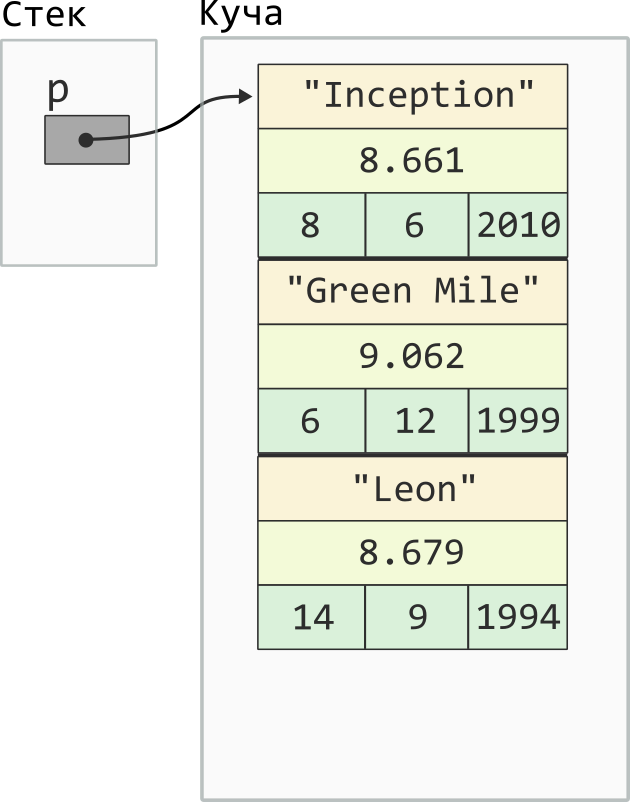
\includegraphics[scale=0.9]{../images/pointer_schemes/pointer_to_array_of_struct_movie_2.png}
\end{center}
\vspace{65ex}
Одна из проблем в коде выше заключается в том, что для поля \texttt{title} всегда
выделяется \texttt{50} байт на стеке. Название фильма обычно значительно меньше, чем \texttt{50} байт, так что 
много памяти выделяется зря. Более того, если вдруг появится фильм с длиной названия более \texttt{50} символов, то такая структура не сможет его обработать. Решение -- выделять память под строки динамически, как это
показано на рисунке ниже. \\
Измените код программы так, чтобы он выделял память под строки 
динамически. Также нужно добавить функцию \texttt{void delete\_movie\_array(Movie* pm)}, которая будет
освобождать всю выделенную под массив структур память (и под строки и под сам массив).


\begin{center}
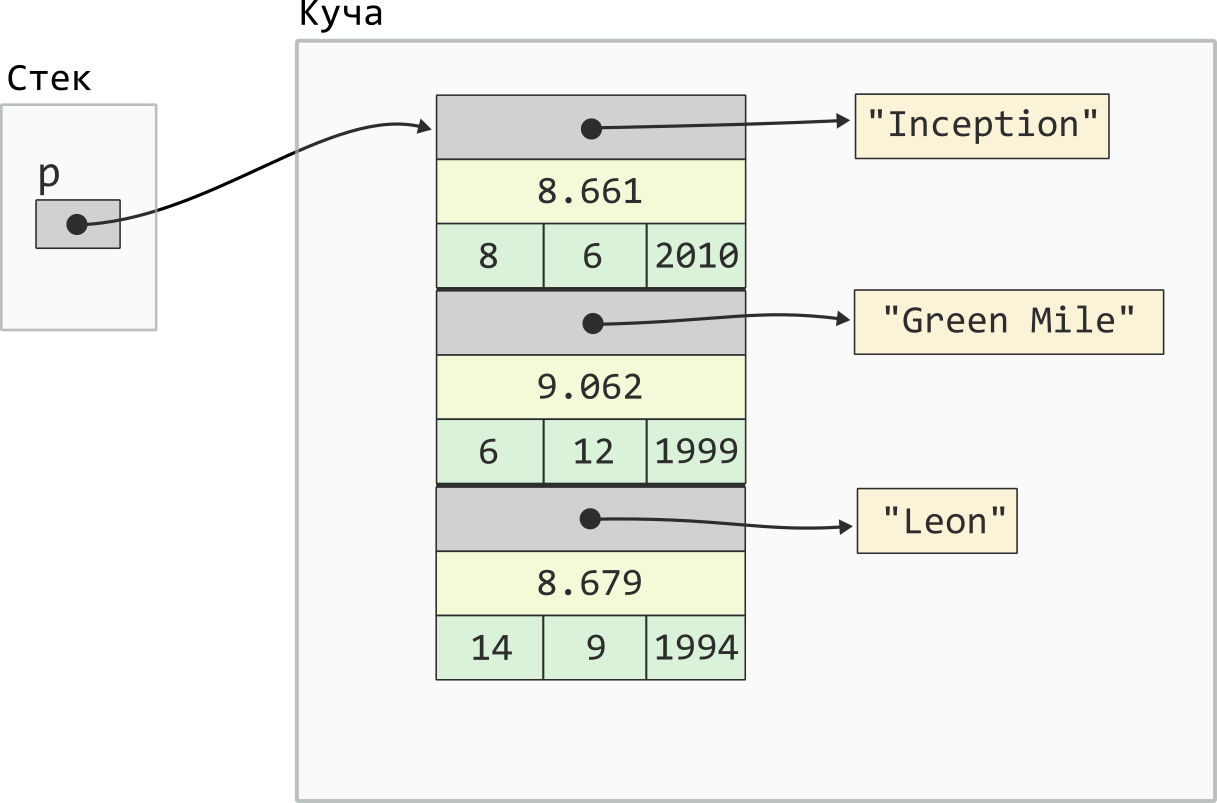
\includegraphics[scale=0.9]{../images/pointer_schemes/pointer_to_array_of_struct_movie_charpointers.png}
\end{center}

\subsection{Двумерный динамический массив}
В стандартной библиотеке нет специальных средств по созданию
двумерных динамических массивов. Есть 2 варианта для создания
такого массива:
\begin{enumerate}
\item Создать одномерный динамический массив размера \texttt{n * m} и работать с ним.
Это хороший вариант, когда длины всех строк массива равны или примерно равны и не меняются.
\item Создать динамический массив из указателей, каждый указатель будет 
соответствовать строке. Затем, для каждой строки динамически выделить столько памяти,
сколько нужно. При этом нам нужно будет создать отдельный массив(\texttt{sizes}), который будет хранить
размеры каждой строки.
\end{enumerate}
\begin{center}
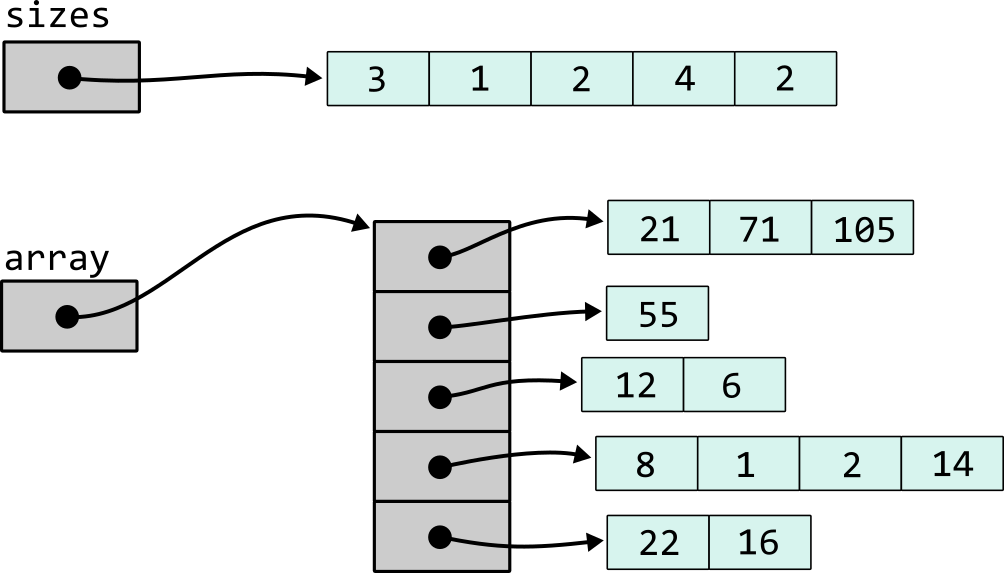
\includegraphics[scale=1]{../images/pointer_schemes/two_dim_dynamic_array.png}
\end{center}
Напишите код, который будет выделять память и инициализировать её в соответствии 
со схемой на рисунке. Также напишите и проверьте функции: \\
\texttt{void print\_two\_dim\_array(int n, int* sizes, int** array)} - печать такого массива и\\
\texttt{void delete\_two\_dim\_array(int n, int* sizes, int** array)} - освобождение памяти.

\subsection{Динамический массив строк}
Динамический массив строк -- это двумерный динамический массив элементов типа \texttt{char}. 
Но с одной особеностью: размер строки задаётся не числом в отдельной переменной, 
а специальным нулевым символом на конце строки. Поэтому от массива \texttt{sizes}
из прошлой задачи можно отказаться.\\

\textbf{Задача \#21:} Пусть есть файл \texttt{words.txt} с примерно следующим содержанием:
\begin{verbatim}
5
Hello
OK
Cat
Antidisestablishmentarianism
Programming
\end{verbatim}
\begin{itemize}
\item Написать функцию \texttt{void read\_words(char* filename, int* p\_number\_of\_words, char*** p\_words)},
которая будет считывать из файла такого формата все слова, выделять в куче память под эти слова и сохранять слова в этой памяти. Вызов этой функции должен происходить таким образом:
\begin{lstlisting}
int number_of_words;
char** words;
read_words("words.txt", &number_of_words, &words);
\end{lstlisting}
Считайте, что каждое слово не превышает \texttt{10000} символов. Также учтите, что при выделении памяти на строку нужно не забывать нулевой символ на конце строки (функция \texttt{strlen} возвращает длину строки без учёта этого символа). 
\item Написать функцию \texttt{void write\_words(FILE* stream, int number\_of\_words, char** words)}, которая будет печатать все слова.

\item Написать функцию \texttt{void sort\_words(int number\_of\_words, char** words)}, которая будет сортировать все слова по адфавиту.

\item Считайте все слова, отсортируйте их и запишите всё в файл \texttt{sorted\_words.txt}. (не забудьте освободить всю память в конце).
\end{itemize}
\end{document}
